% =============================================================================
%  Bayesian Borrowing Methods — Formulations and Illustrations
%  Insert into your main .tex document with % =============================================================================
%  Bayesian Borrowing Methods — Formulations and Illustrations
%  Insert into your main .tex document with % =============================================================================
%  Bayesian Borrowing Methods — Formulations and Illustrations
%  Insert into your main .tex document with % =============================================================================
%  Bayesian Borrowing Methods — Formulations and Illustrations
%  Insert into your main .tex document with \input{bayesian_borrowing}
%  or compile standalone with the preamble below.
% =============================================================================

% ---- Standalone preamble (remove if inserting into an existing document) ----
\documentclass[11pt]{article}
\usepackage{amsmath, amssymb}
\usepackage{graphicx}
\usepackage{booktabs}
\usepackage{geometry}
\usepackage{xcolor}
\usepackage{caption}
\usepackage{hyperref}
\geometry{margin=1in}

\newcommand{\given}{\,|\,}
\newcommand{\propto}{\propto}

\begin{document}
% ---------------------------------------------------------------------------


% =============================================================================
\section*{Bayesian Borrowing Methods}
% =============================================================================

Bayesian borrowing incorporates information from external (historical or
concurrent) data sources into the analysis of a current study.  Let
$\theta$ denote the treatment-effect parameter of interest in the current
study, $D_0$ the external (historical) data, and $D_c$ the current data.
Three widely used strategies are described below.

% -----------------------------------------------------------------------------
\subsection*{1.\; Power Prior}
% -----------------------------------------------------------------------------

\paragraph{Key idea.}
The historical likelihood is down-weighted by a scalar $\alpha \in [0,1]$
before being combined with the initial prior $\pi_0(\theta)$.

\paragraph{Formulation.}

\begin{equation}
  \pi(\theta \given D_0,\,\alpha)
    \;\propto\;
    L(\theta \given D_0)^{\alpha}\,\pi_0(\theta),
  \label{eq:power-prior}
\end{equation}

\noindent where $L(\theta \given D_0)$ is the likelihood of $\theta$ under
the external data and $\alpha$ is fixed or assigned a hyperprior
$p(\alpha)$ (the \emph{normalised} power prior).

\begin{itemize}
  \item $\alpha = 0$: no borrowing — prior reduces to $\pi_0(\theta)$.
  \item $\alpha = 1$: full borrowing — historical data treated as equally
        credible as current data.
  \item $0 < \alpha < 1$: partial borrowing, proportional to $\alpha$.
\end{itemize}

The posterior combining both sources is

\begin{equation}
  \pi(\theta \given D_c, D_0, \alpha)
    \;\propto\;
    L(\theta \given D_c)\;
    L(\theta \given D_0)^{\alpha}\;
    \pi_0(\theta).
\end{equation}

\begin{figure}[ht]
  \centering
  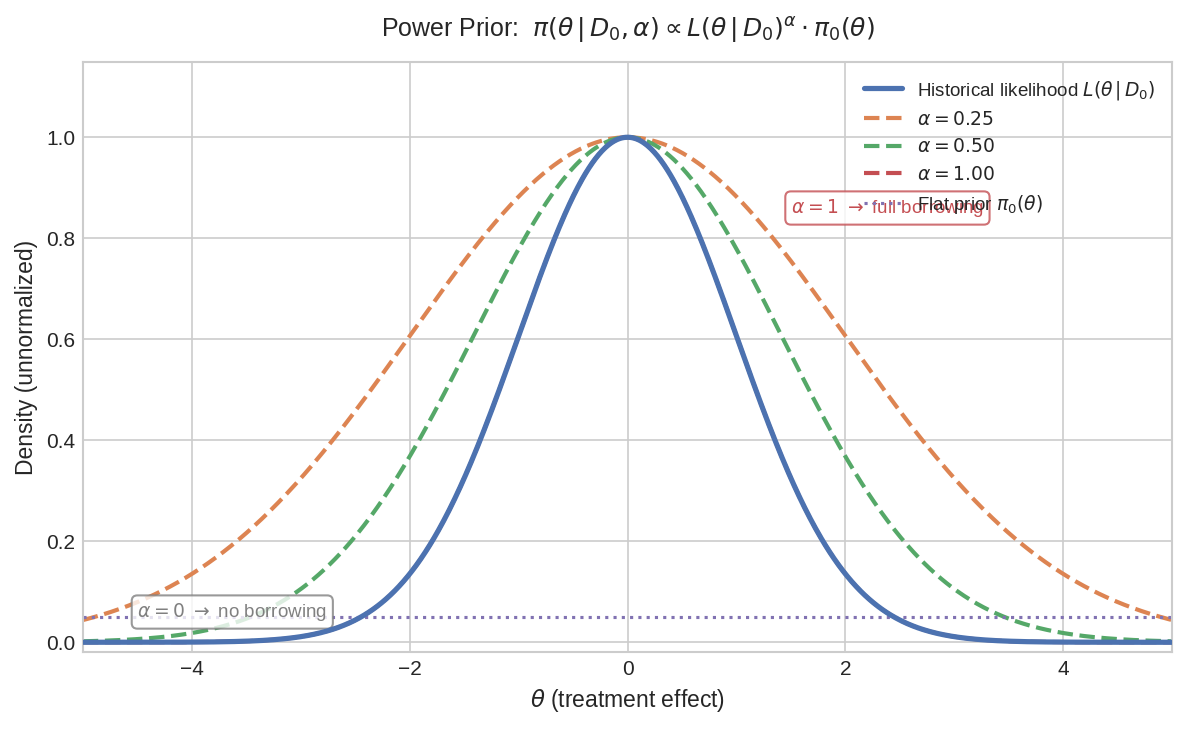
\includegraphics[width=0.75\textwidth]{borrowing_power_prior.png}
  \caption{Power prior: the historical likelihood $L(\theta\given D_0)$
    is raised to the power $\alpha$.  Larger $\alpha$ preserves more of
    the historical information shape; $\alpha=0$ collapses the contribution
    to the flat initial prior.}
  \label{fig:power-prior}
\end{figure}

% -----------------------------------------------------------------------------
\subsection*{2.\; Commensurate Prior}
% -----------------------------------------------------------------------------

\paragraph{Key idea.}
A \emph{commensurability parameter} $\tau > 0$ links the current parameter
$\theta_c$ to the historical estimate $\hat\theta_0$ (or its posterior
$\theta_0$).  The more similar the populations, the larger $\tau$ should
be, and the more the current prior is pulled toward the historical value.

\paragraph{Formulation.}

\begin{equation}
  \theta_c \given \theta_0,\,\tau
    \;\sim\;
    \mathcal{N}\!\left(\theta_0,\;\tau^{-1}\right),
  \label{eq:commensurate}
\end{equation}

\noindent where $\theta_0$ is the historical effect (fixed or itself
given a prior), and $\tau$ may be assigned a hyperprior
$p(\tau)$ to allow data-adaptive borrowing.

\begin{itemize}
  \item Large $\tau$ (populations are commensurate): tight distribution
        around $\theta_0$ — strong borrowing.
  \item Small $\tau$ (populations differ): diffuse distribution — weak
        borrowing.
  \item $\tau \to \infty$: $\theta_c \to \theta_0$ (full borrowing).
  \item $\tau \to 0$: prior on $\theta_c$ becomes flat (no borrowing).
\end{itemize}

The full model is hierarchical:

\begin{align}
  \theta_0   &\;\sim\; \pi_0(\theta_0), \notag \\
  \theta_c \given \theta_0, \tau
             &\;\sim\; \mathcal{N}(\theta_0,\,\tau^{-1}), \label{eq:comm-hier} \\
  D_c \given \theta_c
             &\;\sim\; L(\theta_c \given D_c). \notag
\end{align}

\begin{figure}[ht]
  \centering
  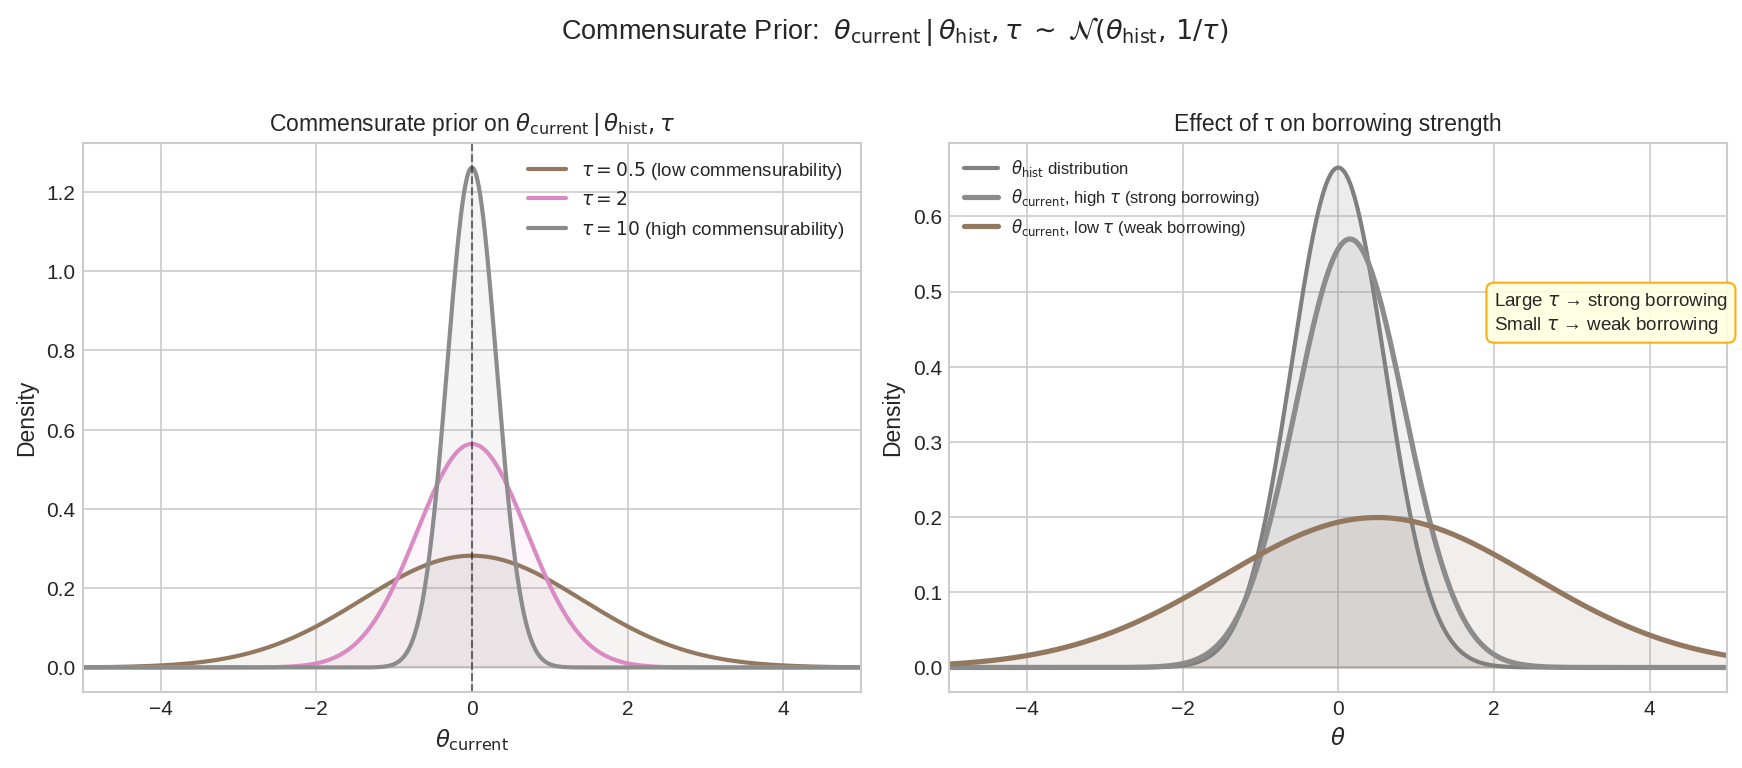
\includegraphics[width=0.80\textwidth]{borrowing_commensurate.png}
  \caption{Commensurate prior: (left) the prior on $\theta_c$ for three
    values of $\tau$; (right) how the posterior of $\theta_c$ shifts
    relative to the historical $\theta_0$ as $\tau$ varies.
    High $\tau$ pulls $\theta_c$ close to $\theta_0$; low $\tau$ allows
    them to diverge.}
  \label{fig:commensurate}
\end{figure}

% -----------------------------------------------------------------------------
\subsection*{3.\; Bayesian Predictive Prior (Meta-Analytic Predictive)}
% -----------------------------------------------------------------------------

\paragraph{Key idea.}
Historical results from $K$ external studies are synthesised through a
hierarchical (random-effects) model.  The marginal distribution of a
\emph{new}, exchangeable study effect — obtained by integrating out the
common mean $\mu$ — serves as the prior for the current study.

\paragraph{Formulation.}

Let $\hat\theta_k$ ($k = 1,\dots,K$) be the historical study estimates,
and assume

\begin{equation}
  \hat\theta_k \given \mu, \sigma^2_k, \tau^2
    \;\sim\;
    \mathcal{N}\!\left(\mu,\;\sigma^2_k + \tau^2\right),
  \label{eq:map-likelihood}
\end{equation}

\noindent where $\sigma^2_k$ is the within-study variance (assumed known)
and $\tau^2$ is the between-study heterogeneity.

The \emph{meta-analytic predictive} (MAP) prior for $\theta_{\text{new}}$
is the predictive distribution marginalised over $\mu$ and $\tau^2$:

\begin{equation}
  \pi_{\text{MAP}}(\theta_{\text{new}})
    \;=\;
    \int \mathcal{N}\!\left(\theta_{\text{new}}\given\mu,\,\tau^2\right)
    \,p(\mu,\tau^2 \given \hat\theta_{1:K})\;
    d\mu\, d\tau^2.
  \label{eq:map-prior}
\end{equation}

\noindent In practice, \eqref{eq:map-prior} is approximated as a finite
mixture of normal distributions (Schmidli et al., 2014):

\begin{equation}
  \pi_{\text{MAP}}(\theta_{\text{new}})
    \;\approx\;
    \sum_{m=1}^{M} w_m \;\mathcal{N}(\theta_{\text{new}}\given\mu_m,\,\sigma^2_m),
  \qquad \sum_{m=1}^{M} w_m = 1.
  \label{eq:map-mixture}
\end{equation}

\begin{itemize}
  \item If the historical studies are very consistent ($\tau^2 \approx 0$),
        the MAP prior is tight and borrowing is strong.
  \item High between-study heterogeneity ($\tau^2$ large) produces a diffuse
        MAP prior — automatic discounting.
  \item A \emph{robust} MAP prior adds a weakly-informative mixture component
        to protect against prior-data conflict.
\end{itemize}

\begin{figure}[ht]
  \centering
  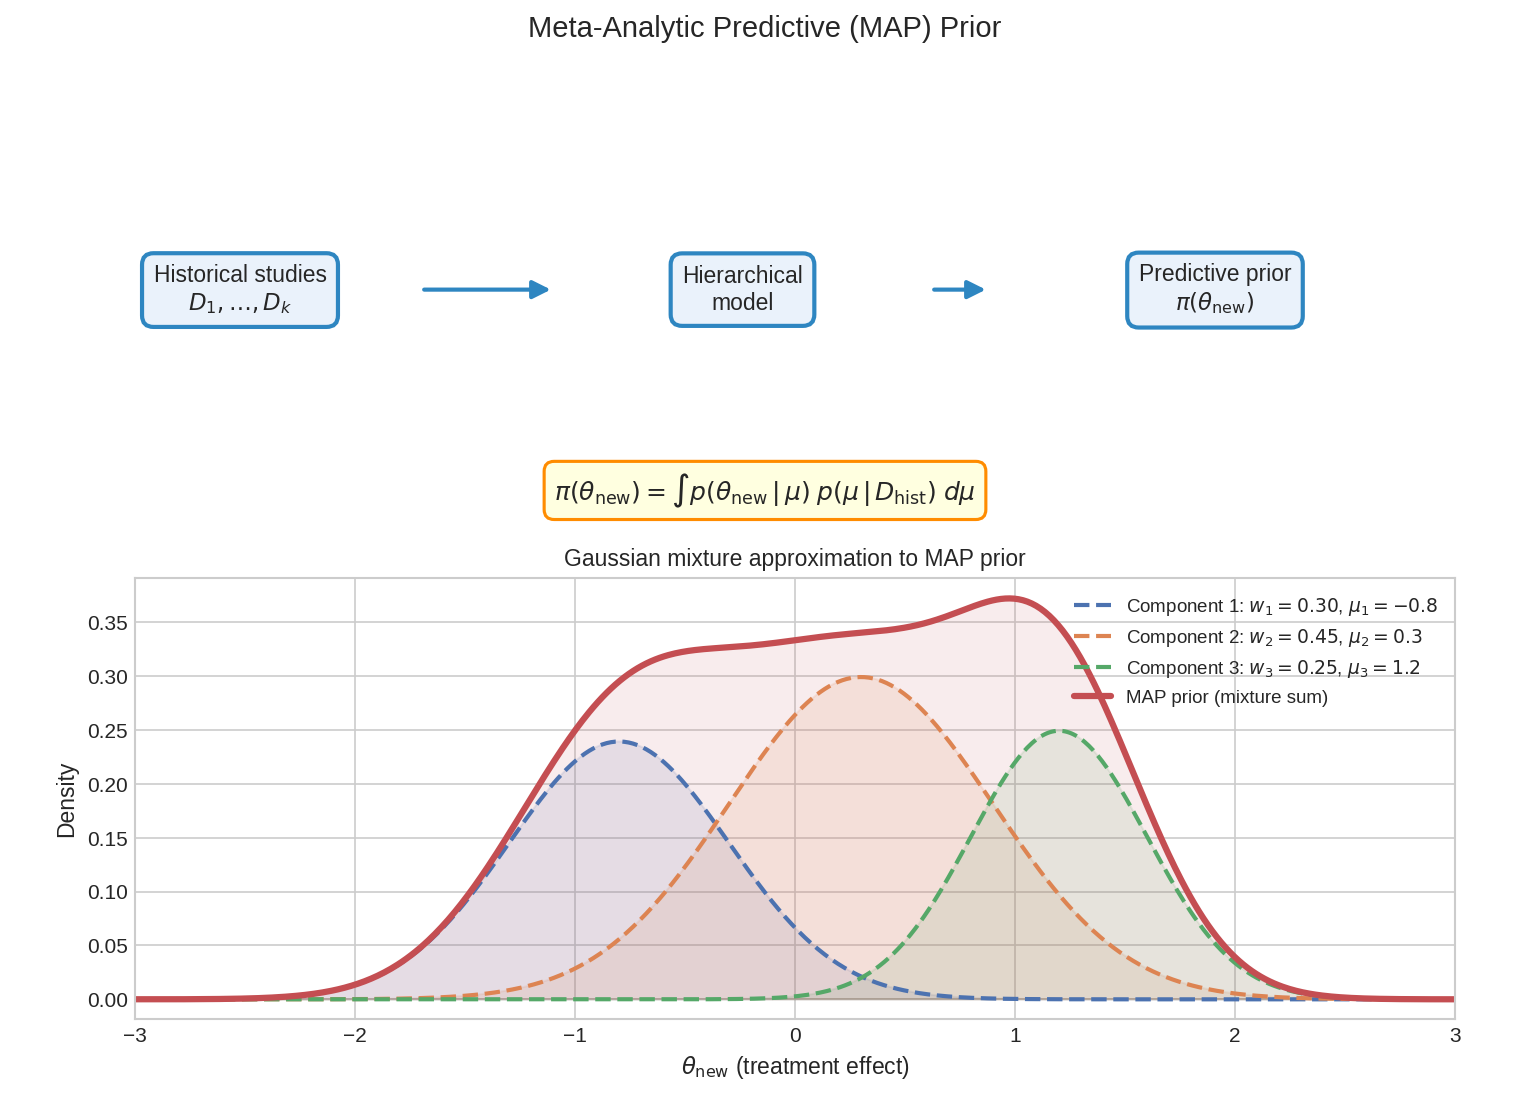
\includegraphics[width=0.78\textwidth]{borrowing_predictive.png}
  \caption{Meta-Analytic Predictive (MAP) prior: historical study estimates
    are fed into a hierarchical model; the predictive distribution for a
    new study effect is approximated as a mixture of Gaussians.}
  \label{fig:map}
\end{figure}

% =============================================================================
\subsection*{Comparison Summary}
% =============================================================================

\begin{table}[ht]
\centering
\caption{Key characteristics of the three Bayesian borrowing methods.}
\label{tab:comparison}
\begin{tabular}{lccc}
\toprule
& \textbf{Power Prior} & \textbf{Commensurate Prior} & \textbf{MAP Prior} \\
\midrule
Borrowing control & $\alpha \in [0,1]$ & $\tau > 0$ & $\tau^2$ (heterogeneity) \\
Mechanism & Weight on $L(θ|D_0)$ & Normal shrinkage to $\theta_0$ & Mixture predictive \\
\# external sources & Single & Single & Multiple \\
Data-adaptive & Optional (hyperprior on $\alpha$) & Yes (hyperprior on $\tau$) & Yes (via $\tau^2$) \\
Conflict detection & Indirect (via $\alpha$) & Indirect (via $\tau$) & Via robust component \\
Computational cost & Low & Moderate & Moderate \\
\bottomrule
\end{tabular}
\end{table}

\begin{figure}[ht]
  \centering
  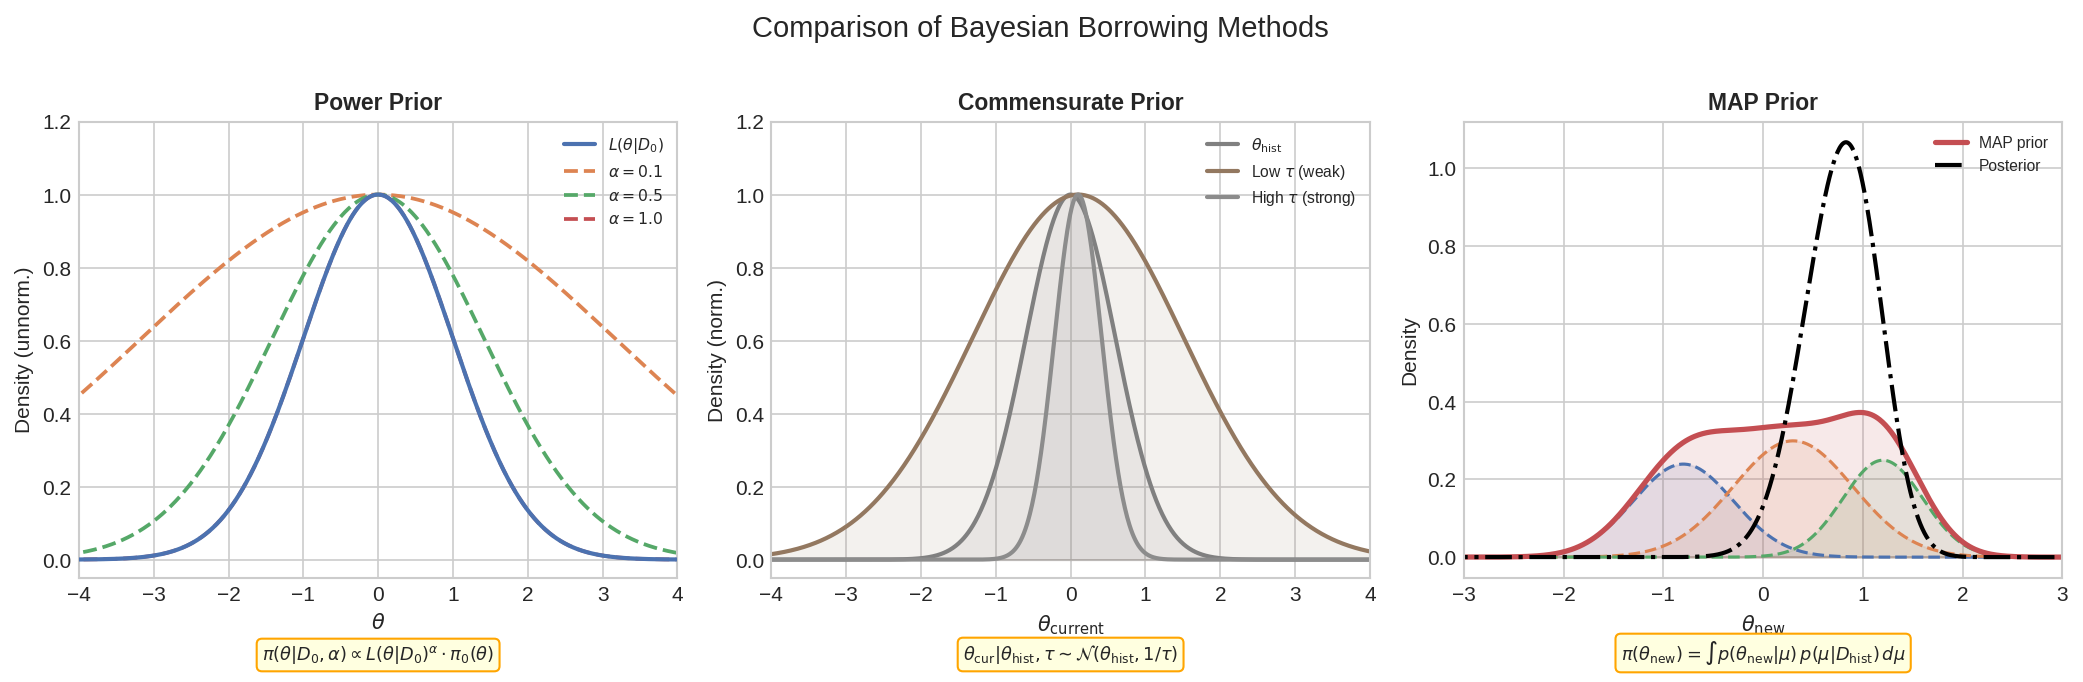
\includegraphics[width=\textwidth]{borrowing_comparison.png}
  \caption{Side-by-side comparison of the three borrowing methods.
    Each panel shows how the borrowing parameter governs the prior placed
    on the current treatment effect $\theta_c$.}
  \label{fig:comparison}
\end{figure}

% ---- End of section (remove \end{document} if inserting into existing file) -
\end{document}

%  or compile standalone with the preamble below.
% =============================================================================

% ---- Standalone preamble (remove if inserting into an existing document) ----
\documentclass[11pt]{article}
\usepackage{amsmath, amssymb}
\usepackage{graphicx}
\usepackage{booktabs}
\usepackage{geometry}
\usepackage{xcolor}
\usepackage{caption}
\usepackage{hyperref}
\geometry{margin=1in}

\newcommand{\given}{\,|\,}
\newcommand{\propto}{\propto}

\begin{document}
% ---------------------------------------------------------------------------


% =============================================================================
\section*{Bayesian Borrowing Methods}
% =============================================================================

Bayesian borrowing incorporates information from external (historical or
concurrent) data sources into the analysis of a current study.  Let
$\theta$ denote the treatment-effect parameter of interest in the current
study, $D_0$ the external (historical) data, and $D_c$ the current data.
Three widely used strategies are described below.

% -----------------------------------------------------------------------------
\subsection*{1.\; Power Prior}
% -----------------------------------------------------------------------------

\paragraph{Key idea.}
The historical likelihood is down-weighted by a scalar $\alpha \in [0,1]$
before being combined with the initial prior $\pi_0(\theta)$.

\paragraph{Formulation.}

\begin{equation}
  \pi(\theta \given D_0,\,\alpha)
    \;\propto\;
    L(\theta \given D_0)^{\alpha}\,\pi_0(\theta),
  \label{eq:power-prior}
\end{equation}

\noindent where $L(\theta \given D_0)$ is the likelihood of $\theta$ under
the external data and $\alpha$ is fixed or assigned a hyperprior
$p(\alpha)$ (the \emph{normalised} power prior).

\begin{itemize}
  \item $\alpha = 0$: no borrowing — prior reduces to $\pi_0(\theta)$.
  \item $\alpha = 1$: full borrowing — historical data treated as equally
        credible as current data.
  \item $0 < \alpha < 1$: partial borrowing, proportional to $\alpha$.
\end{itemize}

The posterior combining both sources is

\begin{equation}
  \pi(\theta \given D_c, D_0, \alpha)
    \;\propto\;
    L(\theta \given D_c)\;
    L(\theta \given D_0)^{\alpha}\;
    \pi_0(\theta).
\end{equation}

\begin{figure}[ht]
  \centering
  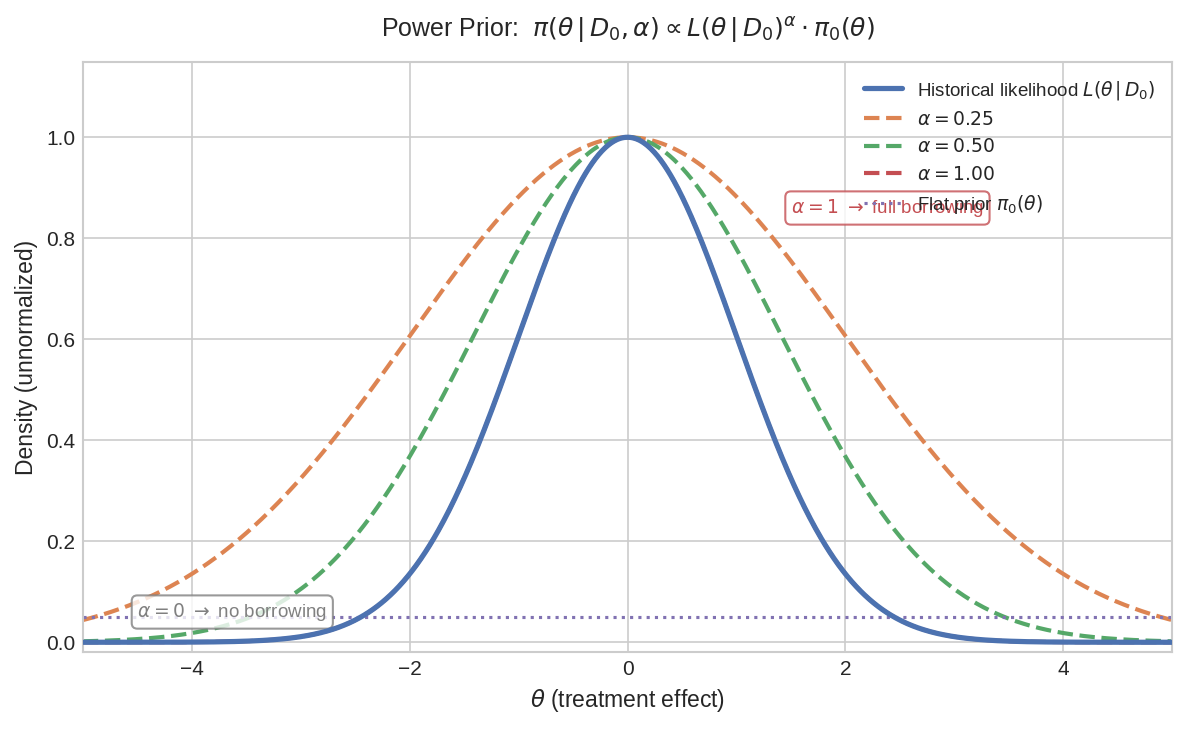
\includegraphics[width=0.75\textwidth]{borrowing_power_prior.png}
  \caption{Power prior: the historical likelihood $L(\theta\given D_0)$
    is raised to the power $\alpha$.  Larger $\alpha$ preserves more of
    the historical information shape; $\alpha=0$ collapses the contribution
    to the flat initial prior.}
  \label{fig:power-prior}
\end{figure}

% -----------------------------------------------------------------------------
\subsection*{2.\; Commensurate Prior}
% -----------------------------------------------------------------------------

\paragraph{Key idea.}
A \emph{commensurability parameter} $\tau > 0$ links the current parameter
$\theta_c$ to the historical estimate $\hat\theta_0$ (or its posterior
$\theta_0$).  The more similar the populations, the larger $\tau$ should
be, and the more the current prior is pulled toward the historical value.

\paragraph{Formulation.}

\begin{equation}
  \theta_c \given \theta_0,\,\tau
    \;\sim\;
    \mathcal{N}\!\left(\theta_0,\;\tau^{-1}\right),
  \label{eq:commensurate}
\end{equation}

\noindent where $\theta_0$ is the historical effect (fixed or itself
given a prior), and $\tau$ may be assigned a hyperprior
$p(\tau)$ to allow data-adaptive borrowing.

\begin{itemize}
  \item Large $\tau$ (populations are commensurate): tight distribution
        around $\theta_0$ — strong borrowing.
  \item Small $\tau$ (populations differ): diffuse distribution — weak
        borrowing.
  \item $\tau \to \infty$: $\theta_c \to \theta_0$ (full borrowing).
  \item $\tau \to 0$: prior on $\theta_c$ becomes flat (no borrowing).
\end{itemize}

The full model is hierarchical:

\begin{align}
  \theta_0   &\;\sim\; \pi_0(\theta_0), \notag \\
  \theta_c \given \theta_0, \tau
             &\;\sim\; \mathcal{N}(\theta_0,\,\tau^{-1}), \label{eq:comm-hier} \\
  D_c \given \theta_c
             &\;\sim\; L(\theta_c \given D_c). \notag
\end{align}

\begin{figure}[ht]
  \centering
  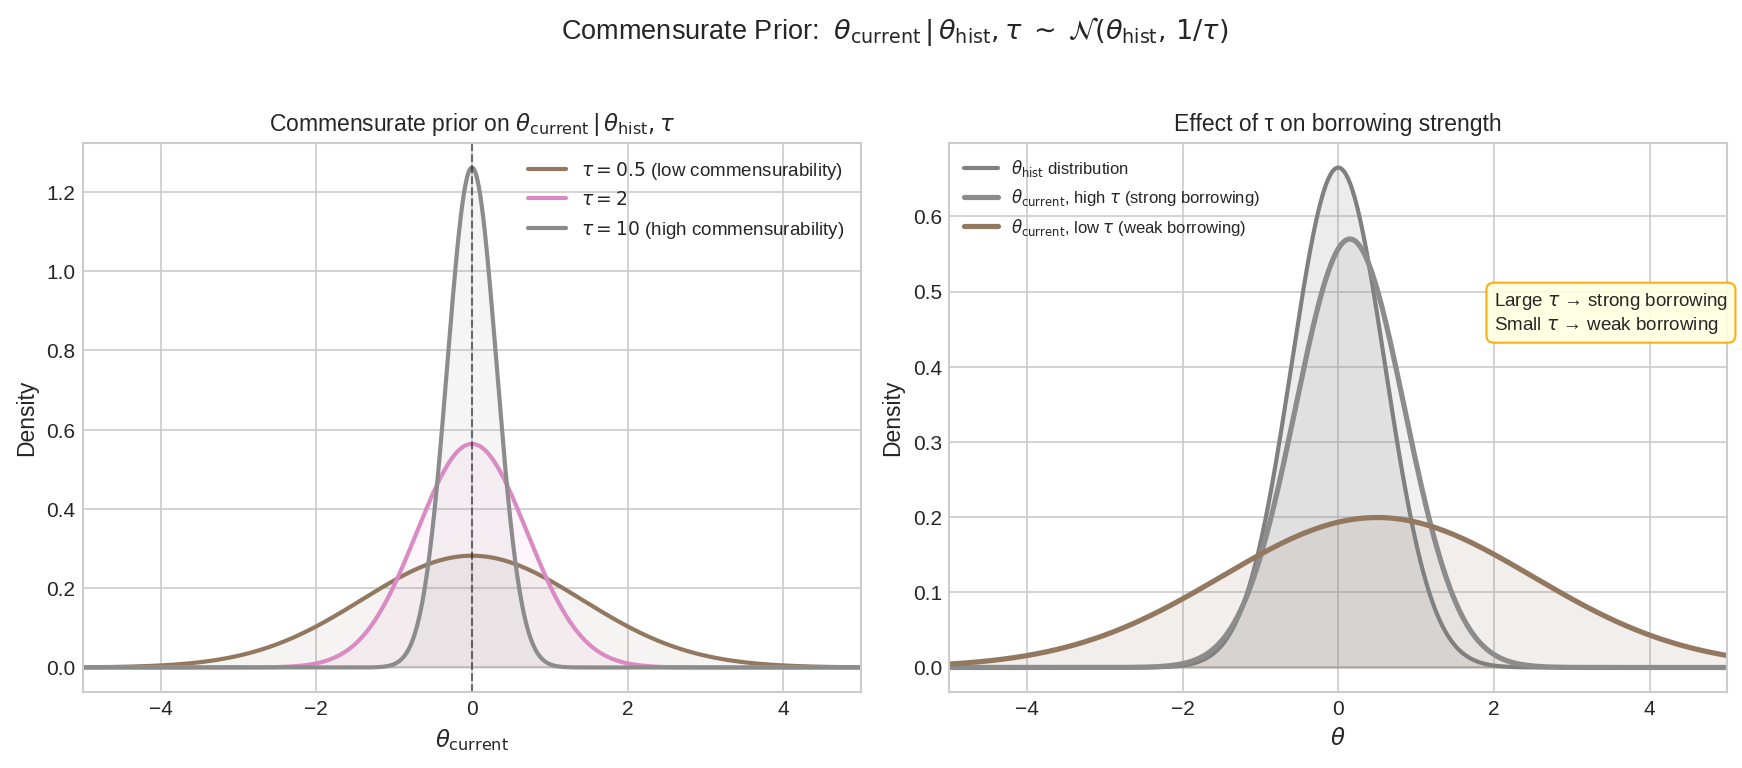
\includegraphics[width=0.80\textwidth]{borrowing_commensurate.png}
  \caption{Commensurate prior: (left) the prior on $\theta_c$ for three
    values of $\tau$; (right) how the posterior of $\theta_c$ shifts
    relative to the historical $\theta_0$ as $\tau$ varies.
    High $\tau$ pulls $\theta_c$ close to $\theta_0$; low $\tau$ allows
    them to diverge.}
  \label{fig:commensurate}
\end{figure}

% -----------------------------------------------------------------------------
\subsection*{3.\; Bayesian Predictive Prior (Meta-Analytic Predictive)}
% -----------------------------------------------------------------------------

\paragraph{Key idea.}
Historical results from $K$ external studies are synthesised through a
hierarchical (random-effects) model.  The marginal distribution of a
\emph{new}, exchangeable study effect — obtained by integrating out the
common mean $\mu$ — serves as the prior for the current study.

\paragraph{Formulation.}

Let $\hat\theta_k$ ($k = 1,\dots,K$) be the historical study estimates,
and assume

\begin{equation}
  \hat\theta_k \given \mu, \sigma^2_k, \tau^2
    \;\sim\;
    \mathcal{N}\!\left(\mu,\;\sigma^2_k + \tau^2\right),
  \label{eq:map-likelihood}
\end{equation}

\noindent where $\sigma^2_k$ is the within-study variance (assumed known)
and $\tau^2$ is the between-study heterogeneity.

The \emph{meta-analytic predictive} (MAP) prior for $\theta_{\text{new}}$
is the predictive distribution marginalised over $\mu$ and $\tau^2$:

\begin{equation}
  \pi_{\text{MAP}}(\theta_{\text{new}})
    \;=\;
    \int \mathcal{N}\!\left(\theta_{\text{new}}\given\mu,\,\tau^2\right)
    \,p(\mu,\tau^2 \given \hat\theta_{1:K})\;
    d\mu\, d\tau^2.
  \label{eq:map-prior}
\end{equation}

\noindent In practice, \eqref{eq:map-prior} is approximated as a finite
mixture of normal distributions (Schmidli et al., 2014):

\begin{equation}
  \pi_{\text{MAP}}(\theta_{\text{new}})
    \;\approx\;
    \sum_{m=1}^{M} w_m \;\mathcal{N}(\theta_{\text{new}}\given\mu_m,\,\sigma^2_m),
  \qquad \sum_{m=1}^{M} w_m = 1.
  \label{eq:map-mixture}
\end{equation}

\begin{itemize}
  \item If the historical studies are very consistent ($\tau^2 \approx 0$),
        the MAP prior is tight and borrowing is strong.
  \item High between-study heterogeneity ($\tau^2$ large) produces a diffuse
        MAP prior — automatic discounting.
  \item A \emph{robust} MAP prior adds a weakly-informative mixture component
        to protect against prior-data conflict.
\end{itemize}

\begin{figure}[ht]
  \centering
  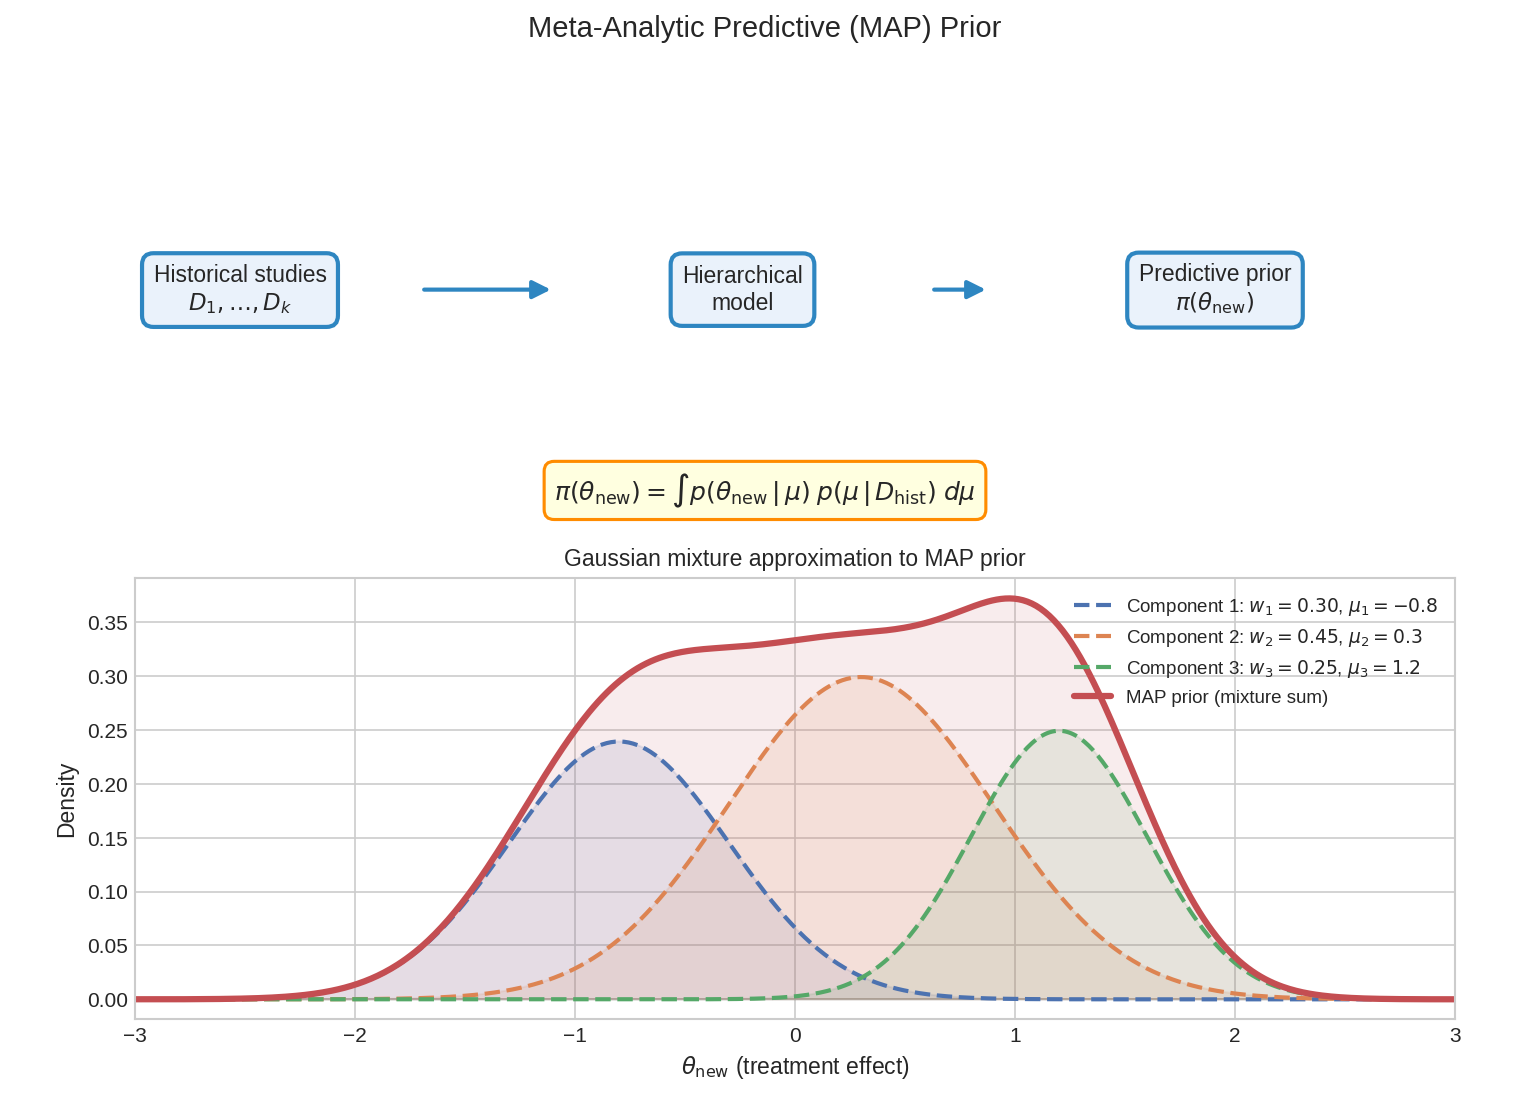
\includegraphics[width=0.78\textwidth]{borrowing_predictive.png}
  \caption{Meta-Analytic Predictive (MAP) prior: historical study estimates
    are fed into a hierarchical model; the predictive distribution for a
    new study effect is approximated as a mixture of Gaussians.}
  \label{fig:map}
\end{figure}

% =============================================================================
\subsection*{Comparison Summary}
% =============================================================================

\begin{table}[ht]
\centering
\caption{Key characteristics of the three Bayesian borrowing methods.}
\label{tab:comparison}
\begin{tabular}{lccc}
\toprule
& \textbf{Power Prior} & \textbf{Commensurate Prior} & \textbf{MAP Prior} \\
\midrule
Borrowing control & $\alpha \in [0,1]$ & $\tau > 0$ & $\tau^2$ (heterogeneity) \\
Mechanism & Weight on $L(θ|D_0)$ & Normal shrinkage to $\theta_0$ & Mixture predictive \\
\# external sources & Single & Single & Multiple \\
Data-adaptive & Optional (hyperprior on $\alpha$) & Yes (hyperprior on $\tau$) & Yes (via $\tau^2$) \\
Conflict detection & Indirect (via $\alpha$) & Indirect (via $\tau$) & Via robust component \\
Computational cost & Low & Moderate & Moderate \\
\bottomrule
\end{tabular}
\end{table}

\begin{figure}[ht]
  \centering
  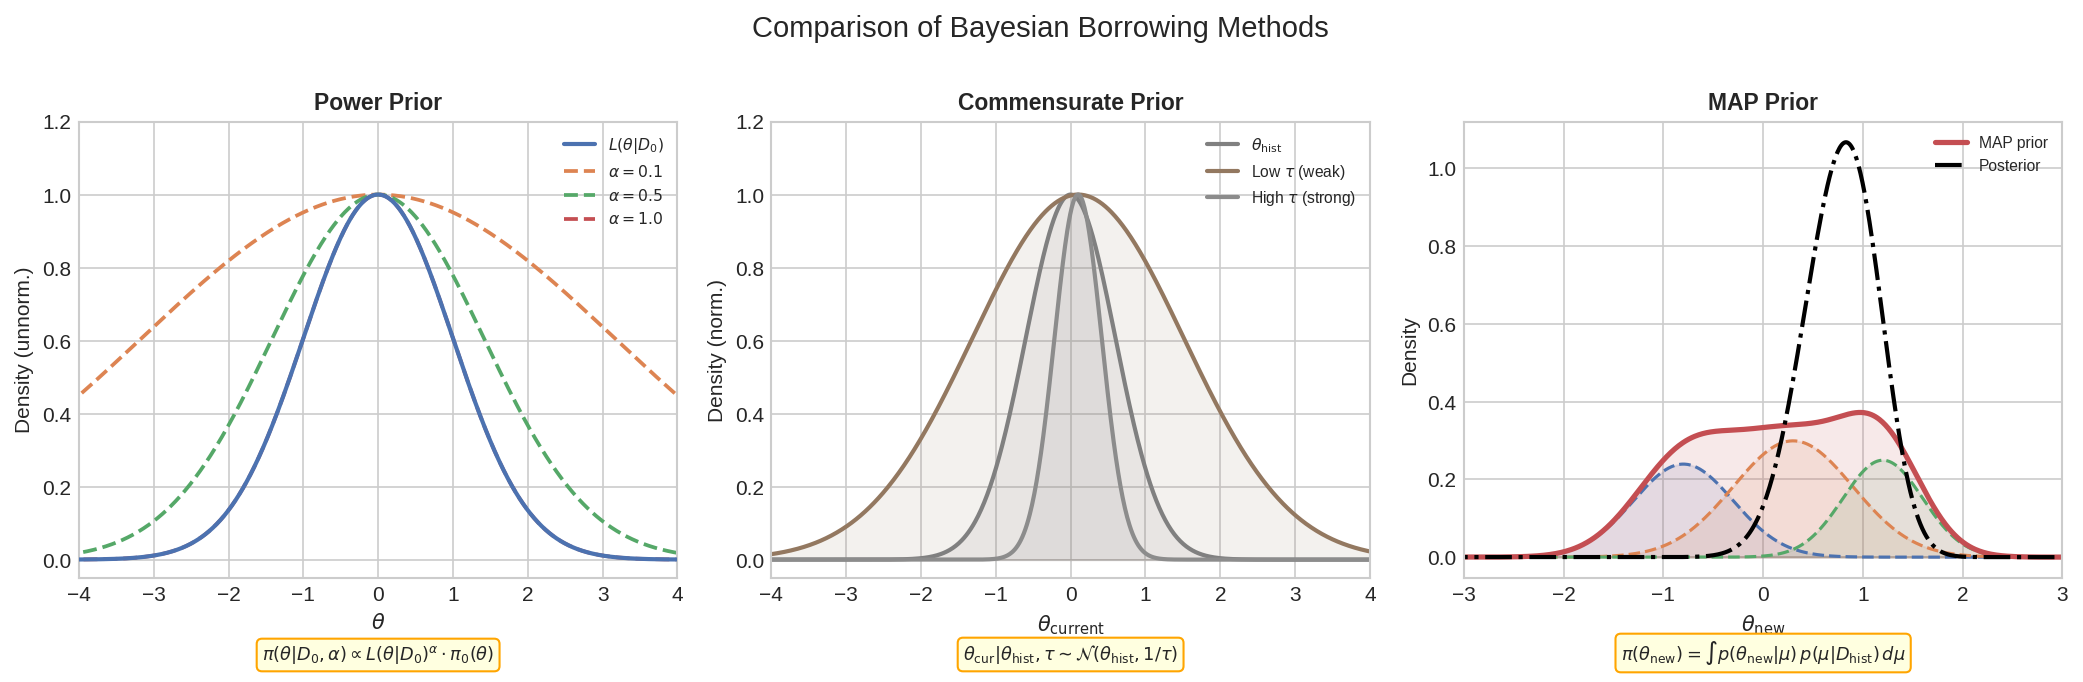
\includegraphics[width=\textwidth]{borrowing_comparison.png}
  \caption{Side-by-side comparison of the three borrowing methods.
    Each panel shows how the borrowing parameter governs the prior placed
    on the current treatment effect $\theta_c$.}
  \label{fig:comparison}
\end{figure}

% ---- End of section (remove \end{document} if inserting into existing file) -
\end{document}

%  or compile standalone with the preamble below.
% =============================================================================

% ---- Standalone preamble (remove if inserting into an existing document) ----
\documentclass[11pt]{article}
\usepackage{amsmath, amssymb}
\usepackage{graphicx}
\usepackage{booktabs}
\usepackage{geometry}
\usepackage{xcolor}
\usepackage{caption}
\usepackage{hyperref}
\geometry{margin=1in}

\newcommand{\given}{\,|\,}
\newcommand{\propto}{\propto}

\begin{document}
% ---------------------------------------------------------------------------


% =============================================================================
\section*{Bayesian Borrowing Methods}
% =============================================================================

Bayesian borrowing incorporates information from external (historical or
concurrent) data sources into the analysis of a current study.  Let
$\theta$ denote the treatment-effect parameter of interest in the current
study, $D_0$ the external (historical) data, and $D_c$ the current data.
Three widely used strategies are described below.

% -----------------------------------------------------------------------------
\subsection*{1.\; Power Prior}
% -----------------------------------------------------------------------------

\paragraph{Key idea.}
The historical likelihood is down-weighted by a scalar $\alpha \in [0,1]$
before being combined with the initial prior $\pi_0(\theta)$.

\paragraph{Formulation.}

\begin{equation}
  \pi(\theta \given D_0,\,\alpha)
    \;\propto\;
    L(\theta \given D_0)^{\alpha}\,\pi_0(\theta),
  \label{eq:power-prior}
\end{equation}

\noindent where $L(\theta \given D_0)$ is the likelihood of $\theta$ under
the external data and $\alpha$ is fixed or assigned a hyperprior
$p(\alpha)$ (the \emph{normalised} power prior).

\begin{itemize}
  \item $\alpha = 0$: no borrowing — prior reduces to $\pi_0(\theta)$.
  \item $\alpha = 1$: full borrowing — historical data treated as equally
        credible as current data.
  \item $0 < \alpha < 1$: partial borrowing, proportional to $\alpha$.
\end{itemize}

The posterior combining both sources is

\begin{equation}
  \pi(\theta \given D_c, D_0, \alpha)
    \;\propto\;
    L(\theta \given D_c)\;
    L(\theta \given D_0)^{\alpha}\;
    \pi_0(\theta).
\end{equation}

\begin{figure}[ht]
  \centering
  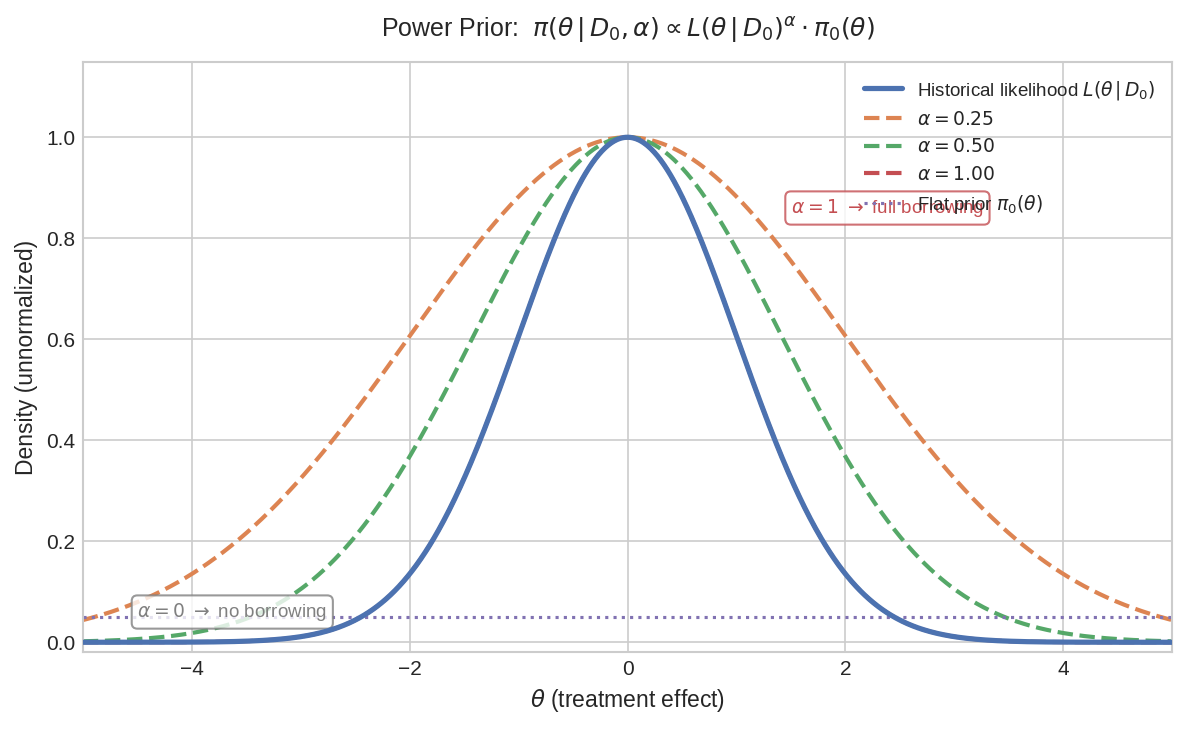
\includegraphics[width=0.75\textwidth]{borrowing_power_prior.png}
  \caption{Power prior: the historical likelihood $L(\theta\given D_0)$
    is raised to the power $\alpha$.  Larger $\alpha$ preserves more of
    the historical information shape; $\alpha=0$ collapses the contribution
    to the flat initial prior.}
  \label{fig:power-prior}
\end{figure}

% -----------------------------------------------------------------------------
\subsection*{2.\; Commensurate Prior}
% -----------------------------------------------------------------------------

\paragraph{Key idea.}
A \emph{commensurability parameter} $\tau > 0$ links the current parameter
$\theta_c$ to the historical estimate $\hat\theta_0$ (or its posterior
$\theta_0$).  The more similar the populations, the larger $\tau$ should
be, and the more the current prior is pulled toward the historical value.

\paragraph{Formulation.}

\begin{equation}
  \theta_c \given \theta_0,\,\tau
    \;\sim\;
    \mathcal{N}\!\left(\theta_0,\;\tau^{-1}\right),
  \label{eq:commensurate}
\end{equation}

\noindent where $\theta_0$ is the historical effect (fixed or itself
given a prior), and $\tau$ may be assigned a hyperprior
$p(\tau)$ to allow data-adaptive borrowing.

\begin{itemize}
  \item Large $\tau$ (populations are commensurate): tight distribution
        around $\theta_0$ — strong borrowing.
  \item Small $\tau$ (populations differ): diffuse distribution — weak
        borrowing.
  \item $\tau \to \infty$: $\theta_c \to \theta_0$ (full borrowing).
  \item $\tau \to 0$: prior on $\theta_c$ becomes flat (no borrowing).
\end{itemize}

The full model is hierarchical:

\begin{align}
  \theta_0   &\;\sim\; \pi_0(\theta_0), \notag \\
  \theta_c \given \theta_0, \tau
             &\;\sim\; \mathcal{N}(\theta_0,\,\tau^{-1}), \label{eq:comm-hier} \\
  D_c \given \theta_c
             &\;\sim\; L(\theta_c \given D_c). \notag
\end{align}

\begin{figure}[ht]
  \centering
  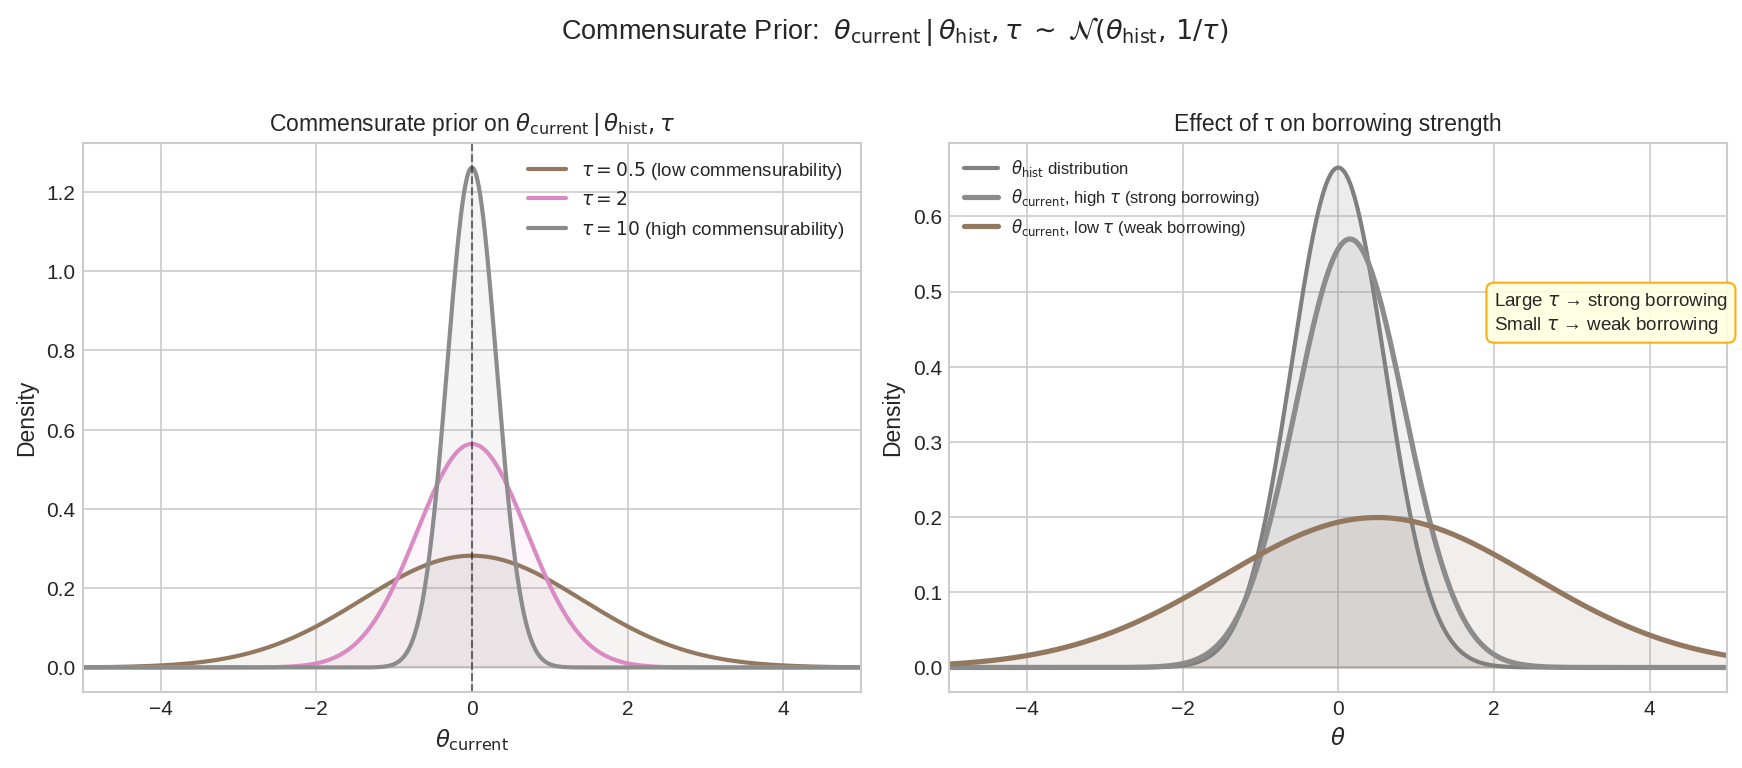
\includegraphics[width=0.80\textwidth]{borrowing_commensurate.png}
  \caption{Commensurate prior: (left) the prior on $\theta_c$ for three
    values of $\tau$; (right) how the posterior of $\theta_c$ shifts
    relative to the historical $\theta_0$ as $\tau$ varies.
    High $\tau$ pulls $\theta_c$ close to $\theta_0$; low $\tau$ allows
    them to diverge.}
  \label{fig:commensurate}
\end{figure}

% -----------------------------------------------------------------------------
\subsection*{3.\; Bayesian Predictive Prior (Meta-Analytic Predictive)}
% -----------------------------------------------------------------------------

\paragraph{Key idea.}
Historical results from $K$ external studies are synthesised through a
hierarchical (random-effects) model.  The marginal distribution of a
\emph{new}, exchangeable study effect — obtained by integrating out the
common mean $\mu$ — serves as the prior for the current study.

\paragraph{Formulation.}

Let $\hat\theta_k$ ($k = 1,\dots,K$) be the historical study estimates,
and assume

\begin{equation}
  \hat\theta_k \given \mu, \sigma^2_k, \tau^2
    \;\sim\;
    \mathcal{N}\!\left(\mu,\;\sigma^2_k + \tau^2\right),
  \label{eq:map-likelihood}
\end{equation}

\noindent where $\sigma^2_k$ is the within-study variance (assumed known)
and $\tau^2$ is the between-study heterogeneity.

The \emph{meta-analytic predictive} (MAP) prior for $\theta_{\text{new}}$
is the predictive distribution marginalised over $\mu$ and $\tau^2$:

\begin{equation}
  \pi_{\text{MAP}}(\theta_{\text{new}})
    \;=\;
    \int \mathcal{N}\!\left(\theta_{\text{new}}\given\mu,\,\tau^2\right)
    \,p(\mu,\tau^2 \given \hat\theta_{1:K})\;
    d\mu\, d\tau^2.
  \label{eq:map-prior}
\end{equation}

\noindent In practice, \eqref{eq:map-prior} is approximated as a finite
mixture of normal distributions (Schmidli et al., 2014):

\begin{equation}
  \pi_{\text{MAP}}(\theta_{\text{new}})
    \;\approx\;
    \sum_{m=1}^{M} w_m \;\mathcal{N}(\theta_{\text{new}}\given\mu_m,\,\sigma^2_m),
  \qquad \sum_{m=1}^{M} w_m = 1.
  \label{eq:map-mixture}
\end{equation}

\begin{itemize}
  \item If the historical studies are very consistent ($\tau^2 \approx 0$),
        the MAP prior is tight and borrowing is strong.
  \item High between-study heterogeneity ($\tau^2$ large) produces a diffuse
        MAP prior — automatic discounting.
  \item A \emph{robust} MAP prior adds a weakly-informative mixture component
        to protect against prior-data conflict.
\end{itemize}

\begin{figure}[ht]
  \centering
  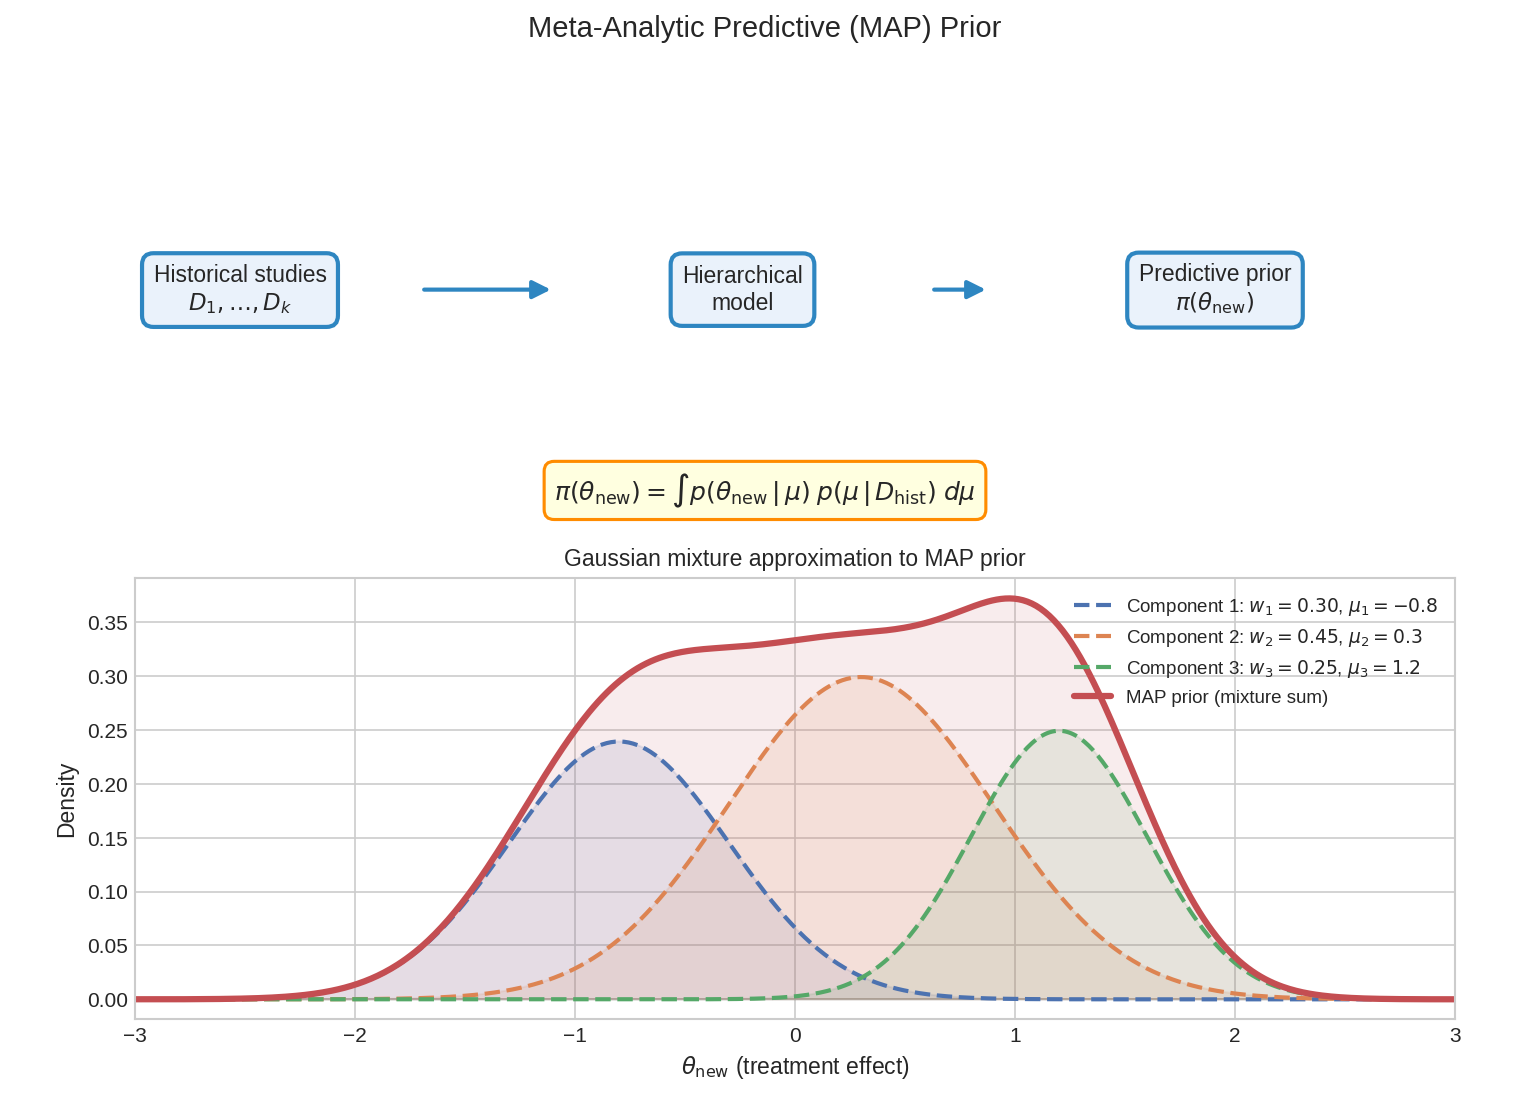
\includegraphics[width=0.78\textwidth]{borrowing_predictive.png}
  \caption{Meta-Analytic Predictive (MAP) prior: historical study estimates
    are fed into a hierarchical model; the predictive distribution for a
    new study effect is approximated as a mixture of Gaussians.}
  \label{fig:map}
\end{figure}

% =============================================================================
\subsection*{Comparison Summary}
% =============================================================================

\begin{table}[ht]
\centering
\caption{Key characteristics of the three Bayesian borrowing methods.}
\label{tab:comparison}
\begin{tabular}{lccc}
\toprule
& \textbf{Power Prior} & \textbf{Commensurate Prior} & \textbf{MAP Prior} \\
\midrule
Borrowing control & $\alpha \in [0,1]$ & $\tau > 0$ & $\tau^2$ (heterogeneity) \\
Mechanism & Weight on $L(θ|D_0)$ & Normal shrinkage to $\theta_0$ & Mixture predictive \\
\# external sources & Single & Single & Multiple \\
Data-adaptive & Optional (hyperprior on $\alpha$) & Yes (hyperprior on $\tau$) & Yes (via $\tau^2$) \\
Conflict detection & Indirect (via $\alpha$) & Indirect (via $\tau$) & Via robust component \\
Computational cost & Low & Moderate & Moderate \\
\bottomrule
\end{tabular}
\end{table}

\begin{figure}[ht]
  \centering
  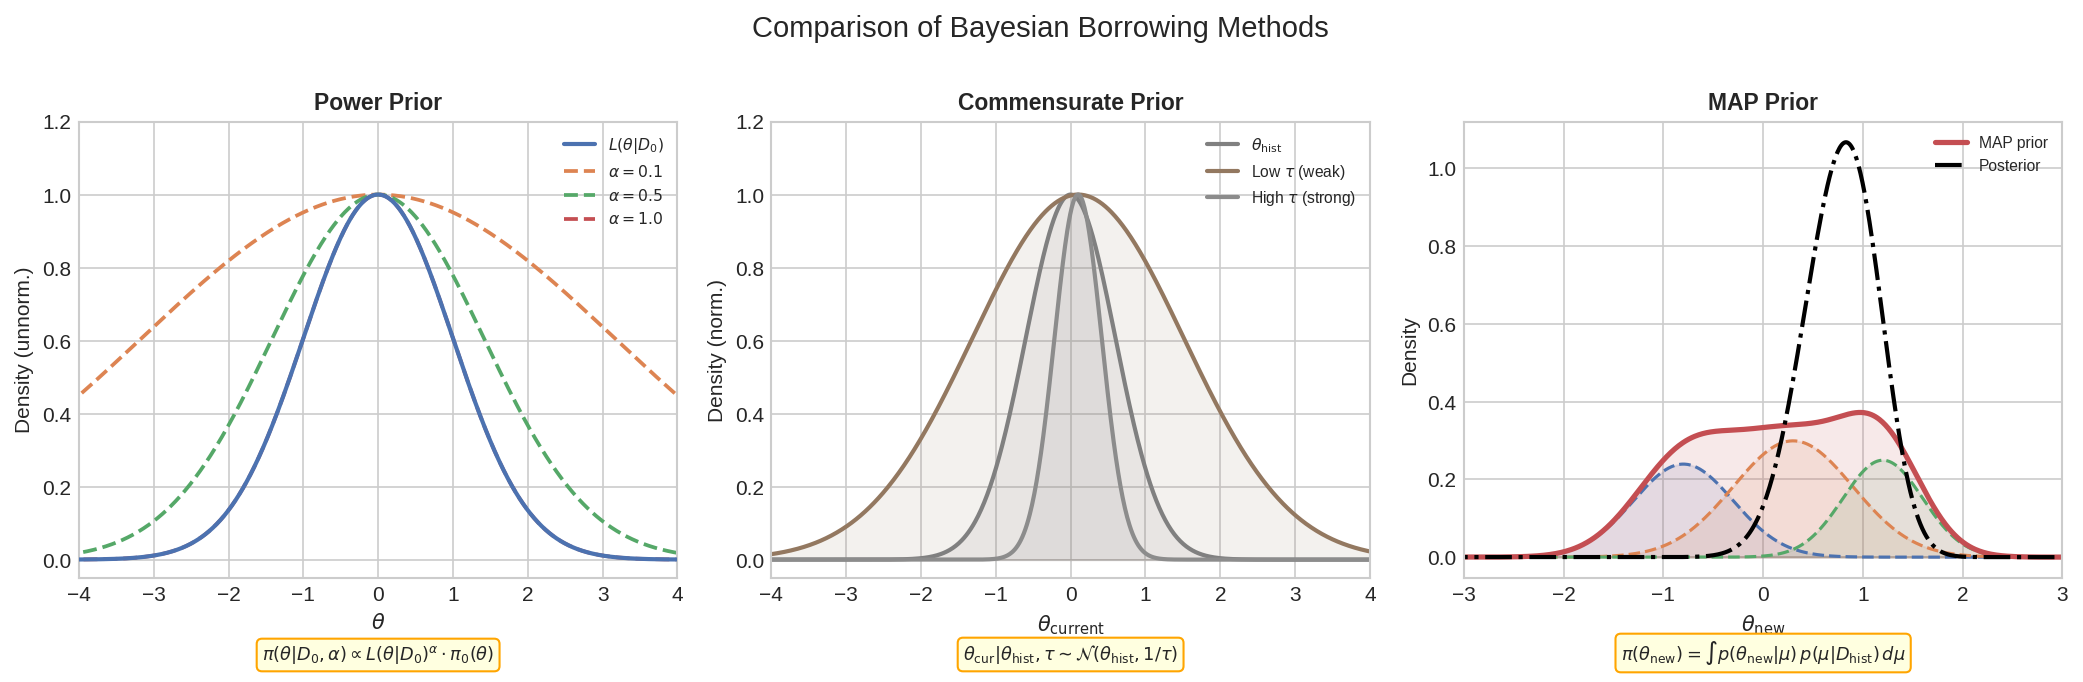
\includegraphics[width=\textwidth]{borrowing_comparison.png}
  \caption{Side-by-side comparison of the three borrowing methods.
    Each panel shows how the borrowing parameter governs the prior placed
    on the current treatment effect $\theta_c$.}
  \label{fig:comparison}
\end{figure}

% ---- End of section (remove \end{document} if inserting into existing file) -
\end{document}

%  or compile standalone with the preamble below.
% =============================================================================

% ---- Standalone preamble (remove if inserting into an existing document) ----
\documentclass[11pt]{article}
\usepackage{amsmath, amssymb}
\usepackage{graphicx}
\usepackage{booktabs}
\usepackage{geometry}
\usepackage{xcolor}
\usepackage{caption}
\usepackage{hyperref}
\geometry{margin=1in}

\newcommand{\given}{\,|\,}
\newcommand{\propto}{\propto}

\begin{document}
% ---------------------------------------------------------------------------


% =============================================================================
\section*{Bayesian Borrowing Methods}
% =============================================================================

Bayesian borrowing incorporates information from external (historical or
concurrent) data sources into the analysis of a current study.  Let
$\theta$ denote the treatment-effect parameter of interest in the current
study, $D_0$ the external (historical) data, and $D_c$ the current data.
Three widely used strategies are described below.

% -----------------------------------------------------------------------------
\subsection*{1.\; Power Prior}
% -----------------------------------------------------------------------------

\paragraph{Key idea.}
The historical likelihood is down-weighted by a scalar $\alpha \in [0,1]$
before being combined with the initial prior $\pi_0(\theta)$.

\paragraph{Formulation.}

\begin{equation}
  \pi(\theta \given D_0,\,\alpha)
    \;\propto\;
    L(\theta \given D_0)^{\alpha}\,\pi_0(\theta),
  \label{eq:power-prior}
\end{equation}

\noindent where $L(\theta \given D_0)$ is the likelihood of $\theta$ under
the external data and $\alpha$ is fixed or assigned a hyperprior
$p(\alpha)$ (the \emph{normalised} power prior).

\begin{itemize}
  \item $\alpha = 0$: no borrowing — prior reduces to $\pi_0(\theta)$.
  \item $\alpha = 1$: full borrowing — historical data treated as equally
        credible as current data.
  \item $0 < \alpha < 1$: partial borrowing, proportional to $\alpha$.
\end{itemize}

The posterior combining both sources is

\begin{equation}
  \pi(\theta \given D_c, D_0, \alpha)
    \;\propto\;
    L(\theta \given D_c)\;
    L(\theta \given D_0)^{\alpha}\;
    \pi_0(\theta).
\end{equation}

\begin{figure}[ht]
  \centering
  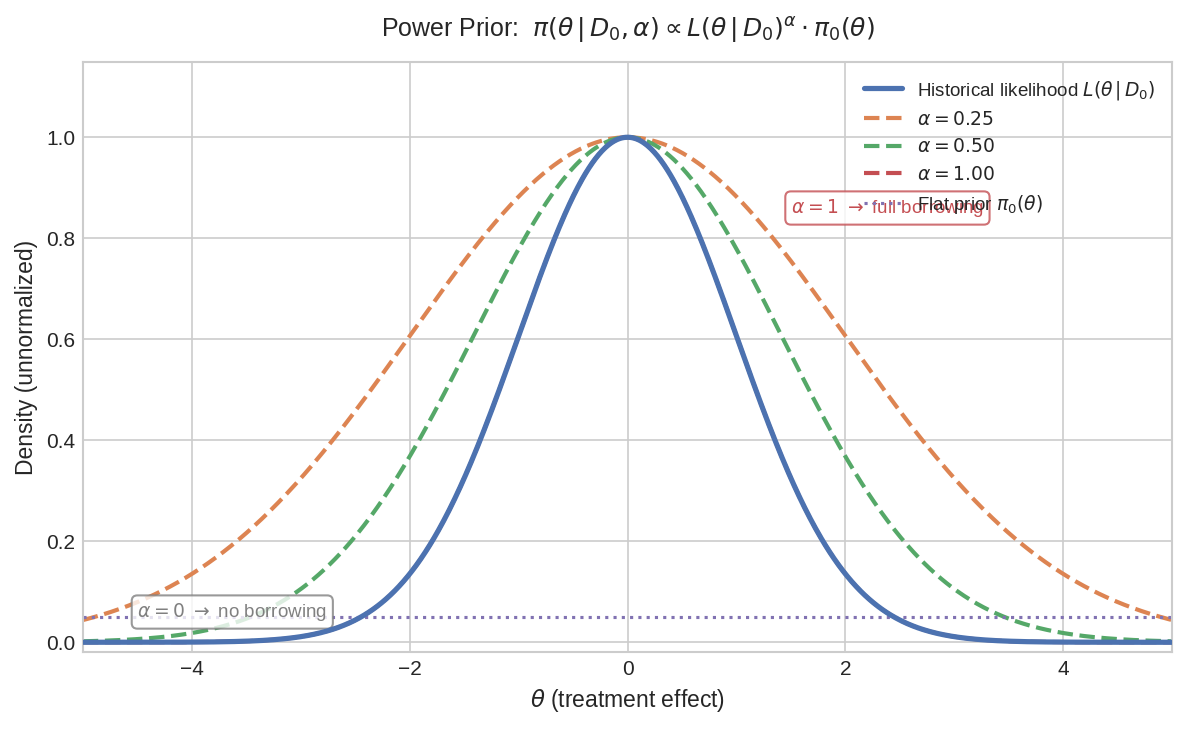
\includegraphics[width=0.75\textwidth]{borrowing_power_prior.png}
  \caption{Power prior: the historical likelihood $L(\theta\given D_0)$
    is raised to the power $\alpha$.  Larger $\alpha$ preserves more of
    the historical information shape; $\alpha=0$ collapses the contribution
    to the flat initial prior.}
  \label{fig:power-prior}
\end{figure}

% -----------------------------------------------------------------------------
\subsection*{2.\; Commensurate Prior}
% -----------------------------------------------------------------------------

\paragraph{Key idea.}
A \emph{commensurability parameter} $\tau > 0$ links the current parameter
$\theta_c$ to the historical estimate $\hat\theta_0$ (or its posterior
$\theta_0$).  The more similar the populations, the larger $\tau$ should
be, and the more the current prior is pulled toward the historical value.

\paragraph{Formulation.}

\begin{equation}
  \theta_c \given \theta_0,\,\tau
    \;\sim\;
    \mathcal{N}\!\left(\theta_0,\;\tau^{-1}\right),
  \label{eq:commensurate}
\end{equation}

\noindent where $\theta_0$ is the historical effect (fixed or itself
given a prior), and $\tau$ may be assigned a hyperprior
$p(\tau)$ to allow data-adaptive borrowing.

\begin{itemize}
  \item Large $\tau$ (populations are commensurate): tight distribution
        around $\theta_0$ — strong borrowing.
  \item Small $\tau$ (populations differ): diffuse distribution — weak
        borrowing.
  \item $\tau \to \infty$: $\theta_c \to \theta_0$ (full borrowing).
  \item $\tau \to 0$: prior on $\theta_c$ becomes flat (no borrowing).
\end{itemize}

The full model is hierarchical:

\begin{align}
  \theta_0   &\;\sim\; \pi_0(\theta_0), \notag \\
  \theta_c \given \theta_0, \tau
             &\;\sim\; \mathcal{N}(\theta_0,\,\tau^{-1}), \label{eq:comm-hier} \\
  D_c \given \theta_c
             &\;\sim\; L(\theta_c \given D_c). \notag
\end{align}

\begin{figure}[ht]
  \centering
  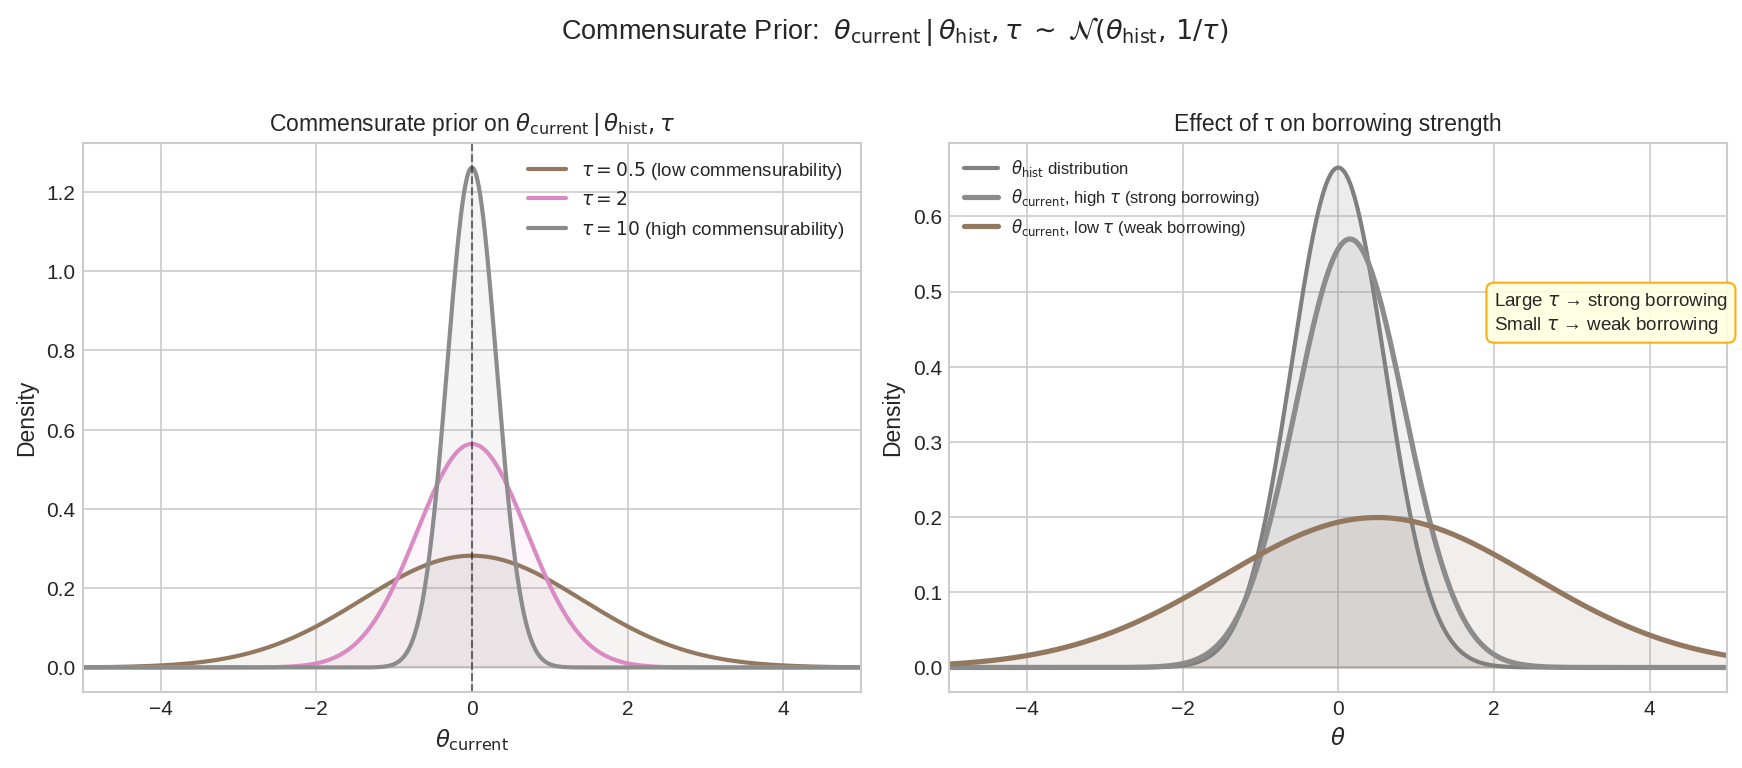
\includegraphics[width=0.80\textwidth]{borrowing_commensurate.png}
  \caption{Commensurate prior: (left) the prior on $\theta_c$ for three
    values of $\tau$; (right) how the posterior of $\theta_c$ shifts
    relative to the historical $\theta_0$ as $\tau$ varies.
    High $\tau$ pulls $\theta_c$ close to $\theta_0$; low $\tau$ allows
    them to diverge.}
  \label{fig:commensurate}
\end{figure}

% -----------------------------------------------------------------------------
\subsection*{3.\; Bayesian Predictive Prior (Meta-Analytic Predictive)}
% -----------------------------------------------------------------------------

\paragraph{Key idea.}
Historical results from $K$ external studies are synthesised through a
hierarchical (random-effects) model.  The marginal distribution of a
\emph{new}, exchangeable study effect — obtained by integrating out the
common mean $\mu$ — serves as the prior for the current study.

\paragraph{Formulation.}

Let $\hat\theta_k$ ($k = 1,\dots,K$) be the historical study estimates,
and assume

\begin{equation}
  \hat\theta_k \given \mu, \sigma^2_k, \tau^2
    \;\sim\;
    \mathcal{N}\!\left(\mu,\;\sigma^2_k + \tau^2\right),
  \label{eq:map-likelihood}
\end{equation}

\noindent where $\sigma^2_k$ is the within-study variance (assumed known)
and $\tau^2$ is the between-study heterogeneity.

The \emph{meta-analytic predictive} (MAP) prior for $\theta_{\text{new}}$
is the predictive distribution marginalised over $\mu$ and $\tau^2$:

\begin{equation}
  \pi_{\text{MAP}}(\theta_{\text{new}})
    \;=\;
    \int \mathcal{N}\!\left(\theta_{\text{new}}\given\mu,\,\tau^2\right)
    \,p(\mu,\tau^2 \given \hat\theta_{1:K})\;
    d\mu\, d\tau^2.
  \label{eq:map-prior}
\end{equation}

\noindent In practice, \eqref{eq:map-prior} is approximated as a finite
mixture of normal distributions (Schmidli et al., 2014):

\begin{equation}
  \pi_{\text{MAP}}(\theta_{\text{new}})
    \;\approx\;
    \sum_{m=1}^{M} w_m \;\mathcal{N}(\theta_{\text{new}}\given\mu_m,\,\sigma^2_m),
  \qquad \sum_{m=1}^{M} w_m = 1.
  \label{eq:map-mixture}
\end{equation}

\begin{itemize}
  \item If the historical studies are very consistent ($\tau^2 \approx 0$),
        the MAP prior is tight and borrowing is strong.
  \item High between-study heterogeneity ($\tau^2$ large) produces a diffuse
        MAP prior — automatic discounting.
  \item A \emph{robust} MAP prior adds a weakly-informative mixture component
        to protect against prior-data conflict.
\end{itemize}

\begin{figure}[ht]
  \centering
  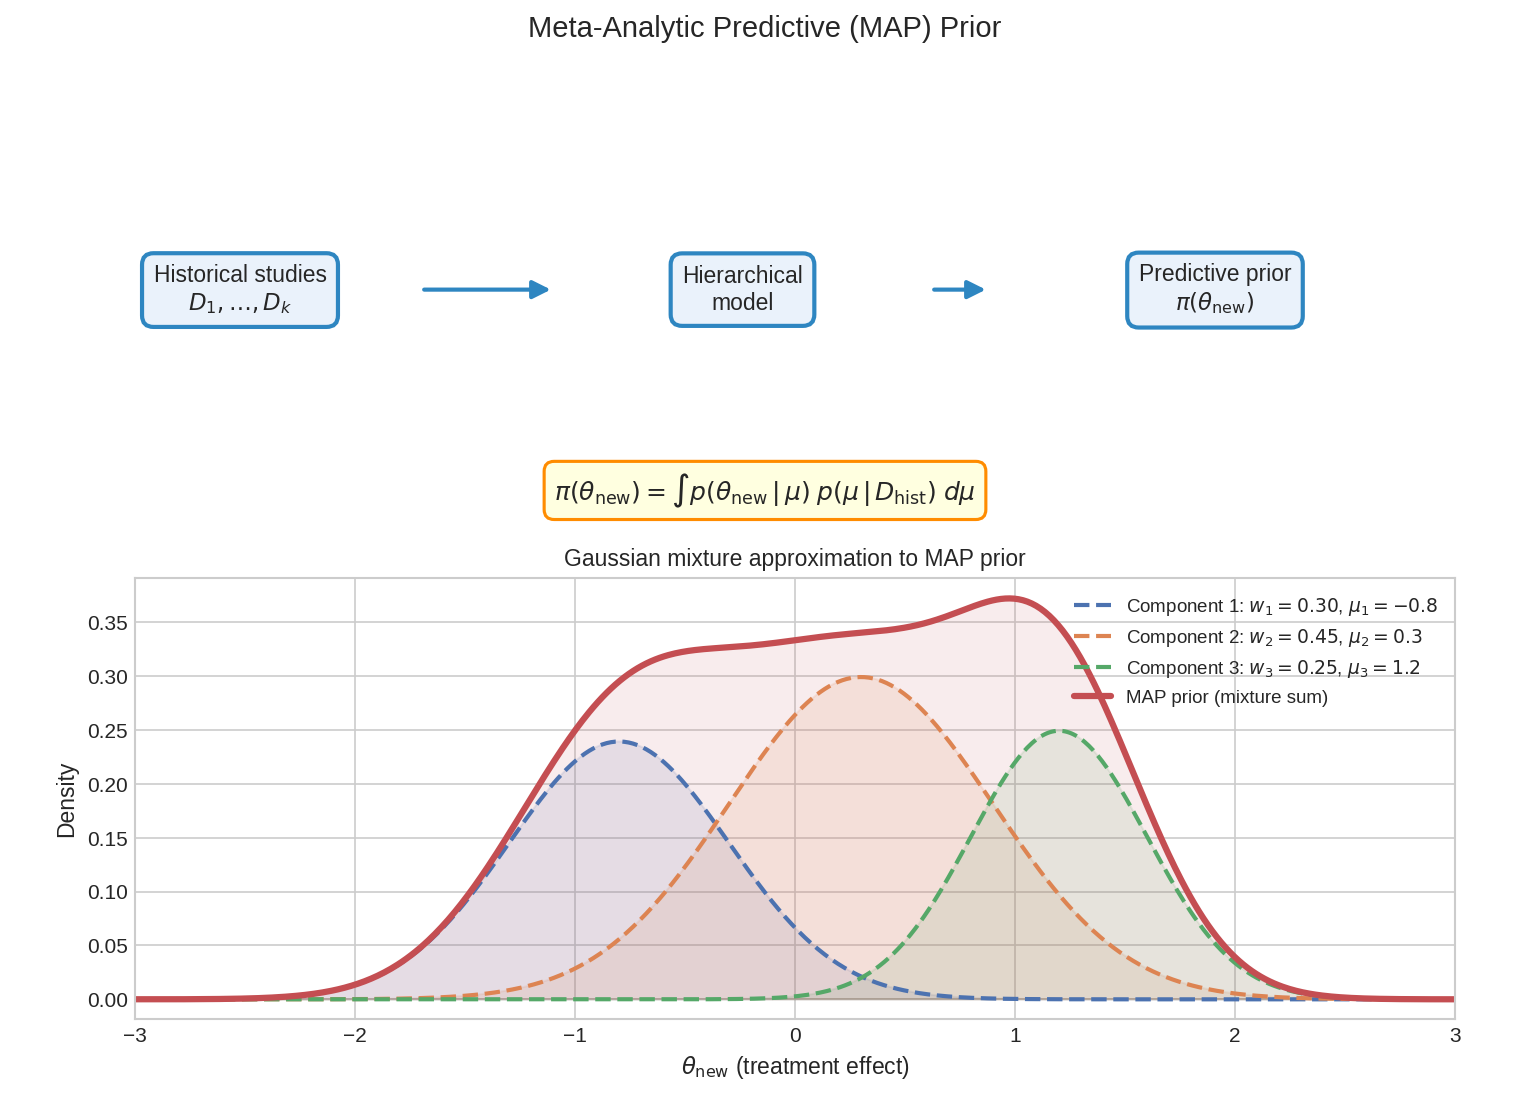
\includegraphics[width=0.78\textwidth]{borrowing_predictive.png}
  \caption{Meta-Analytic Predictive (MAP) prior: historical study estimates
    are fed into a hierarchical model; the predictive distribution for a
    new study effect is approximated as a mixture of Gaussians.}
  \label{fig:map}
\end{figure}

% =============================================================================
\subsection*{Comparison Summary}
% =============================================================================

\begin{table}[ht]
\centering
\caption{Key characteristics of the three Bayesian borrowing methods.}
\label{tab:comparison}
\begin{tabular}{lccc}
\toprule
& \textbf{Power Prior} & \textbf{Commensurate Prior} & \textbf{MAP Prior} \\
\midrule
Borrowing control & $\alpha \in [0,1]$ & $\tau > 0$ & $\tau^2$ (heterogeneity) \\
Mechanism & Weight on $L(θ|D_0)$ & Normal shrinkage to $\theta_0$ & Mixture predictive \\
\# external sources & Single & Single & Multiple \\
Data-adaptive & Optional (hyperprior on $\alpha$) & Yes (hyperprior on $\tau$) & Yes (via $\tau^2$) \\
Conflict detection & Indirect (via $\alpha$) & Indirect (via $\tau$) & Via robust component \\
Computational cost & Low & Moderate & Moderate \\
\bottomrule
\end{tabular}
\end{table}

\begin{figure}[ht]
  \centering
  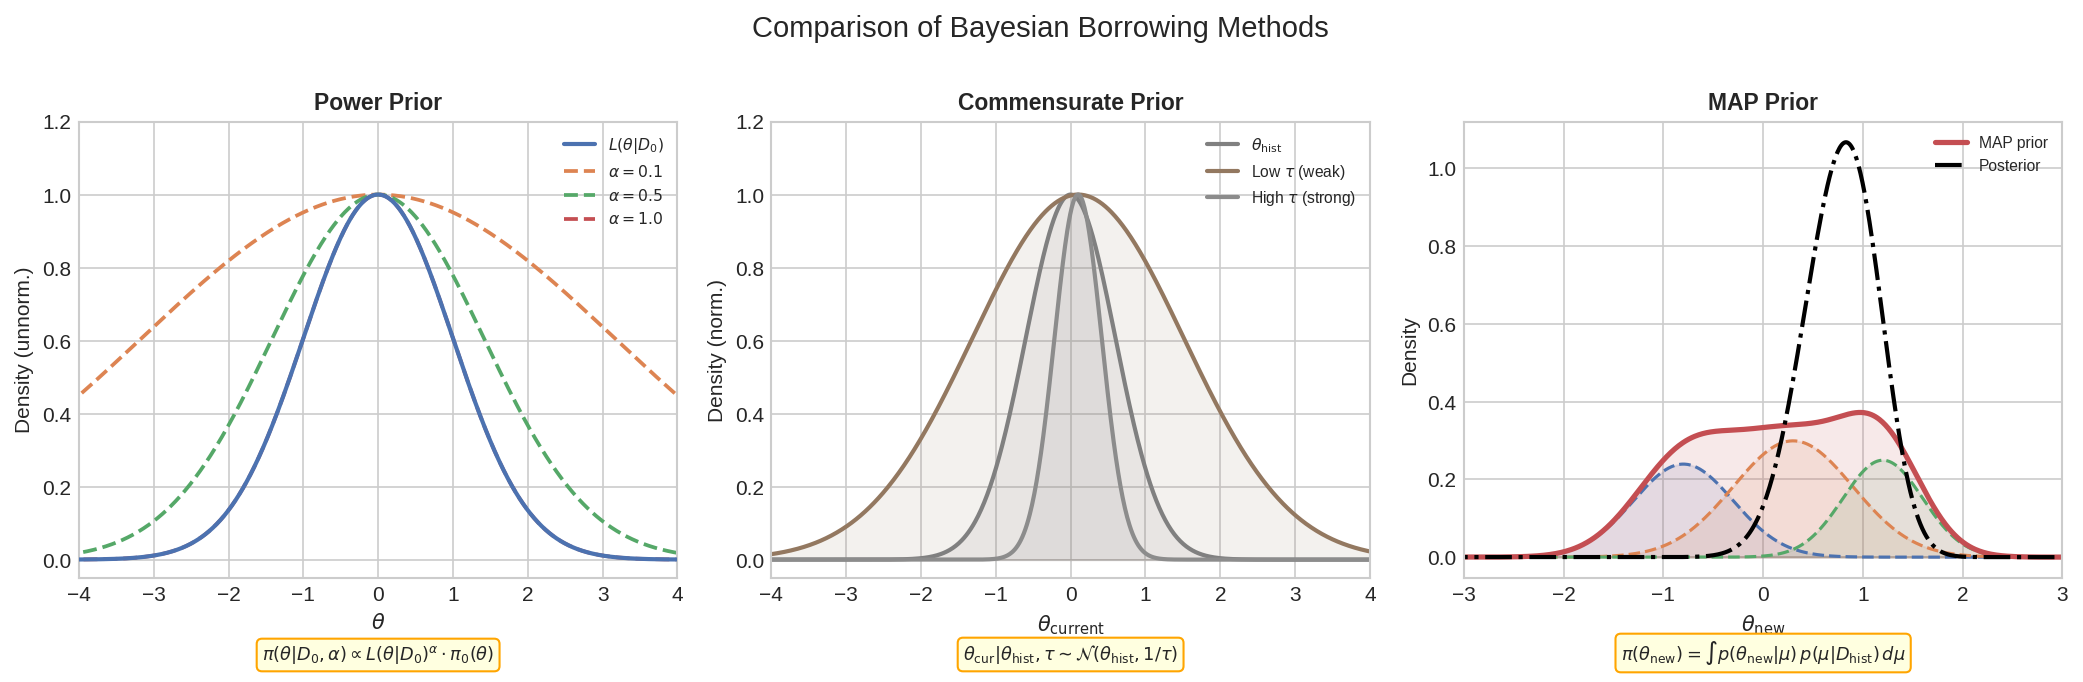
\includegraphics[width=\textwidth]{borrowing_comparison.png}
  \caption{Side-by-side comparison of the three borrowing methods.
    Each panel shows how the borrowing parameter governs the prior placed
    on the current treatment effect $\theta_c$.}
  \label{fig:comparison}
\end{figure}

% ---- End of section (remove \end{document} if inserting into existing file) -
\end{document}
